
%% bare_conf.tex
%% V1.3
%% 2007/01/11
%% by Michael Shell
%% See:
%% http://www.michaelshell.org/
%% for current contact information.
%%
%% This is a skeleton file demonstrating the use of IEEEtran.cls
%% (requires IEEEtran.cls version 1.7 or later) with an IEEE conference paper.
%%
%% Support sites:
%% http://www.michaelshell.org/tex/ieeetran/
%% http://www.ctan.org/tex-archive/macros/latex/contrib/IEEEtran/
%% and
%% http://www.ieee.org/

%%*************************************************************************
%% Legal Notice:
%% This code is offered as-is without any warranty either expressed or
%% implied; without even the implied warranty of MERCHANTABILITY or
%% FITNESS FOR A PARTICULAR PURPOSE! 
%% User assumes all risk.
%% In no event shall IEEE or any contributor to this code be liable for
%% any damages or losses, including, but not limited to, incidental,
%% consequential, or any other damages, resulting from the use or misuse
%% of any information contained here.
%%
%% All comments are the opinions of their respective authors and are not
%% necessarily endorsed by the IEEE.
%%
%% This work is distributed under the LaTeX Project Public License (LPPL)
%% ( http://www.latex-project.org/ ) version 1.3, and may be freely used,
%% distributed and modified. A copy of the LPPL, version 1.3, is included
%% in the base LaTeX documentation of all distributions of LaTeX released
%% 2003/12/01 or later.
%% Retain all contribution notices and credits.
%% ** Modified files should be clearly indicated as such, including  **
%% ** renaming them and changing author support contact information. **
%%
%% File list of work: IEEEtran.cls, IEEEtran_HOWTO.pdf, bare_adv.tex,
%%                    bare_conf.tex, bare_jrnl.tex, bare_jrnl_compsoc.tex
%%*************************************************************************

% *** Authors should verify (and, if needed, correct) their LaTeX system  ***
% *** with the testflow diagnostic prior to trusting their LaTeX platform ***
% *** with production work. IEEE's font choices can trigger bugs that do  ***
% *** not appear when using other class files.                            ***
% The testflow support page is at:
% http://www.michaelshell.org/tex/testflow/



% Note that the a4paper option is mainly intended so that authors in
% countries using A4 can easily print to A4 and see how their papers will
% look in print - the typesetting of the document will not typically be
% affected with changes in paper size (but the bottom and side margins will).
% Use the testflow package mentioned above to verify correct handling of
% both paper sizes by the user's LaTeX system.
%
% Also note that the "draftcls" or "draftclsnofoot", not "draft", option
% should be used if it is desired that the figures are to be displayed in
% draft mode.
%
\documentclass[conference]{IEEEtran}
% Add the compsoc option for Computer Society conferences.
%
% If IEEEtran.cls has not been installed into the LaTeX system files,
% manually specify the path to it like:
% \documentclass[conference]{../sty/IEEEtran}





% Some very useful LaTeX packages include:
% (uncomment the ones you want to load)


% *** MISC UTILITY PACKAGES ***
%
%\usepackage{ifpdf}
% Heiko Oberdiek's ifpdf.sty is very useful if you need conditional
% compilation based on whether the output is pdf or dvi.
% usage:
% \ifpdf
%   % pdf code
% \else
%   % dvi code
% \fi
% The latest version of ifpdf.sty can be obtained from:
% http://www.ctan.org/tex-archive/macros/latex/contrib/oberdiek/
% Also, note that IEEEtran.cls V1.7 and later provides a builtin
% \ifCLASSINFOpdf conditional that works the same way.
% When switching from latex to pdflatex and vice-versa, the compiler may
% have to be run twice to clear warning/error messages.






% *** CITATION PACKAGES ***
%
%\usepackage{cite}
% cite.sty was written by Donald Arseneau
% V1.6 and later of IEEEtran pre-defines the format of the cite.sty package
% \cite{} output to follow that of IEEE. Loading the cite package will
% result in citation numbers being automatically sorted and properly
% "compressed/ranged". e.g., [1], [9], [2], [7], [5], [6] without using
% cite.sty will become [1], [2], [5]--[7], [9] using cite.sty. cite.sty's
% \cite will automatically add leading space, if needed. Use cite.sty's
% noadjust option (cite.sty V3.8 and later) if you want to turn this off.
% cite.sty is already installed on most LaTeX systems. Be sure and use
% version 4.0 (2003-05-27) and later if using hyperref.sty. cite.sty does
% not currently provide for hyperlinked citations.
% The latest version can be obtained at:
% http://www.ctan.org/tex-archive/macros/latex/contrib/cite/
% The documentation is contained in the cite.sty file itself.






% *** GRAPHICS RELATED PACKAUntitled FolderGES ***
%
% Added to commands
\input epsf
\usepackage{graphicx}
\usepackage{hyperref}
\usepackage{graphicx}
\usepackage{amssymb}
\usepackage{amsmath}
\usepackage[super]{nth}
\ifCLASSINFOpdf
  % \usepackage[pdftex]{graphicx}
  % declare the path(s) where your graphic files are
  % \graphicspath{{../pdf/}{../jpeg/}}
  % and their extensions so you won't have to specify these with
  % every instance of \includegraphics
  % \DeclareGraphicsExtensions{.pdf,.jpeg,.png}
\else
  % or other class option (dvipsone, dvipdf, if not using dvips). graphicx
  % will default to the driver specified in the system graphics.cfg if no
  % driver is specified.
  % \usepackage[dvips]{graphicx}
  % declare the path(s) where your graphic files are
  % \graphicspath{{../eps/}}
  % and their extensions so you won't have to specify these with
  % every instance of \includegraphics
  % \DeclareGraphicsExtensions{.eps}
\fi
% graphicx was written by David Carlisle and Sebastian Rahtz. It is
% required if you want graphics, photos, etc. graphicx.sty is already
% installed on most LaTeX systems. The latest version and documentation can
% be obtained at: 
% http://www.ctan.org/tex-archive/macros/latex/required/graphics/
% Another good source of documentation is "Using Imported Graphics in
% LaTeX2e" by Keith Reckdahl which can be found as epslatex.ps or
% epslatex.pdf at: http://www.ctan.org/tex-archive/info/
%
% latex, and pdflatex in dvi mode, support graphics in encapsulated
% postscript (.eps) format. pdflatex in pdf mode supports graphics
% in .pdf, .jpeg, .png and .mps (metapost) formats. Users should ensure
% that all non-photo figures use a vector format (.eps, .pdf, .mps) and
% not a bitmapped formats (.jpeg, .png). IEEE frowns on bitmapped formats
% which can result in "jaggedy"/blurry rendering of lines and letters as
% well as large increases in file sizes.
%
% You can find documentation about the pdfTeX application at:
% http://www.tug.org/applications/pdftex





% *** MATH PACKAGES ***
%
%\usepackage[cmex10]{amsmath}
% A popular package from the American Mathematical Society that provides
% many useful and powerful commands for dealing with mathematics. If using
% it, be sure to load this package with the cmex10 option to ensure that
% only type 1 fonts will utilized at all point sizes. Without this option,
% it is possible that some math symbols, particularly those within
% footnotes, will be rendered in bitmap form which will result in a
% document that can not be IEEE Xplore compliant!
%
% Also, note that the amsmath package sets \interdisplaylinepenalty to 10000
% thus preventing page breaks from occurring within multiline equations. Use:
%\interdisplaylinepenalty=2500
% after loading amsmath to restore such page breaks as IEEEtran.cls normally
% does. amsmath.sty is already installed on most LaTeX systems. The latest
% version and documentation can be obtained at:
% http://www.ctan.org/tex-archive/macros/latex/required/amslatex/math/





% *** SPECIALIZED LIST PACKAGES ***
%
%\usepackage{algorithmic}
% algorithmic.sty was written by Peter Williams and Rogerio Brito.
% This package provides an algorithmic environment fo describing algorithms.
% You can use the algorithmic environment in-text or within a figure
% environment to provide for a floating algorithm. Do NOT use the algorithm
% floating environment provided by algorithm.sty (by the same authors) or
% algorithm2e.sty (by Christophe Fiorio) as IEEE does not use dedicated
% algorithm float types and packages that provide these will not provide
% correct IEEE style captions. The latest version and documentation of
% algorithmic.sty can be obtained at:
% http://www.ctan.org/tex-archive/macros/latex/contrib/algorithms/
% There is also a support site at:
% http://algorithms.berlios.de/index.html
% Also of interest may be the (relatively newer and more customizable)
% algorithmicx.sty package by Szasz Janos:
% http://www.ctan.org/tex-archive/macros/latex/contrib/algorithmicx/




% *** ALIGNMENT PACKAGES ***
%
%\usepackage{array}
% Frank Mittelbach's and David Carlisle's array.sty patches and improves
% the standard LaTeX2e array and tabular environments to provide better
% appearance and additional user controls. As the default LaTeX2e table
% generation code is lacking to the point of almost being broken with
% respect to the quality of the end results, all users are strongly
% advised to use an enhanced (at the very least that provided by array.sty)
% set of table tools. array.sty is already installed on most systems. The
% latest version and documentation can be obtained at:
% http://www.ctan.org/tex-archive/macros/latex/required/tools/


%\usepackage{mdwmath}
%\usepackage{mdwtab}
% Also highly recommended is Mark Wooding's extremely powerful MDW tools,
% especially mdwmath.sty and mdwtab.sty which are used to format equations
% and tables, respectively. The MDWtools set is already installed on most
% LaTeX systems. The lastest version and documentation is available at:
% http://www.ctan.org/tex-archive/macros/latex/contrib/mdwtools/


% IEEEtran contains the IEEEeqnarray family of commands that can be used to
% generate multiline equations as well as matrices, tables, etc., of high
% quality.


%\usepackage{eqparbox}
% Also of notable interest is Scott Pakin's eqparbox package for creating
% (automatically sized) equal width boxes - aka "natural width parboxes".
% Available at:
% http://www.ctan.org/tex-archive/macros/latex/contrib/eqparbox/





% *** SUBFIGURE PACKAGES ***
%\usepackage[tight,footnotesize]{subfigure}
% subfigure.sty was written by Steven Douglas Cochran. This package makes it
% easy to put subfigures in your figures. e.g., "Figure 1a and 1b". For IEEE
% work, it is a good idea to load it with the tight package option to reduce
% the amount of white space around the subfigures. subfigure.sty is already
% installed on most LaTeX systems. The latest version and documentation can
% be obtained at:
% http://www.ctan.org/tex-archive/obsolete/macros/latex/contrib/subfigure/
% subfigure.sty has been superceeded by subfig.sty.



%\usepackage[caption=false]{caption}
%\usepackage[font=footnotesize]{subfig}
% subfig.sty, also written by Steven Douglas Cochran, is the modern
% replacement for subfigure.sty. However, subfig.sty requires and
% automatically loads Axel Sommerfeldt's caption.sty which will override
% IEEEtran.cls handling of captions and this will result in nonIEEE style
% figure/table captions. To prevent this problem, be sure and preload
% caption.sty with its "caption=false" package option. This is will preserve
% IEEEtran.cls handing of captions. Version 1.3 (2005/06/28) and later 
% (recommended due to many improvements over 1.2) of subfig.sty supports
% the caption=false option directly:
%\usepackage[caption=false,font=footnotesize]{subfig}
%
% The latest version and documentation can be obtained at:
% http://www.ctan.org/tex-archive/macros/latex/contrib/subfig/
% The latest version and documentation of caption.sty can be obtained at:
% http://www.ctan.org/tex-archive/macros/latex/contrib/caption/




% *** FLOAT PACKAGES ***
%
%\usepackage{fixltx2e}
% fixltx2e, the successor to the earlier fix2col.sty, was written by
% Frank Mittelbach and David Carlisle. This package corrects a few problems
% in the LaTeX2e kernel, the most notable of which is that in current
% LaTeX2e releases, the ordering of single and double column floats is not
% guaranteed to be preserved. Thus, an unpatched LaTeX2e can allow a
% single column figure to be placed prior to an earlier double column
% figure. The latest version and documentation can be found at:
% http://www.ctan.org/tex-archive/macros/latex/base/



%\usepackage{stfloats}
% stfloats.sty was written by Sigitas Tolusis. This package gives LaTeX2e
% the ability to do double column floats at the bottom of the page as well
% as the top. (e.g., "\begin{figure*}[!b]" is not normally possible in
% LaTeX2e). It also provides a command:
%\fnbelowfloat
% to enable the placement of footnotes below bottom floats (the standard
% LaTeX2e kernel puts them above bottom floats). This is an invasive package
% which rewrites many portions of the LaTeX2e float routines. It may not work
% with other packages that modify the LaTeX2e float routines. The latest
% version and documentation can be obtained at:
% http://www.ctan.org/tex-archive/macros/latex/contrib/sttools/
% Documentation is contained in the stfloats.sty comments as well as in the
% presfull.pdf file. Do not use the stfloats baselinefloat ability as IEEE
% does not allow \baselineskip to stretch. Authors submitting work to the
% IEEE should note that IEEE rarely uses double column equations and
% that authors should try to avoid such use. Do not be tempted to use the
% cuted.sty or midfloat.sty packages (also by Sigitas Tolusis) as IEEE does
% not format its papers in such ways.





% *** PDF, URL AND HYPERLINK PACKAGES ***
%
%\usepackage{url}
% url.sty was written by Donald Arseneau. It provides better support for
% handling and breaking URLs. url.sty is already installed on most LaTeX
% systems. The latest version can be obtained at:
% http://www.ctan.org/tex-archive/macros/latex/contrib/misc/
% Read the url.sty source comments for usage information. Basically,
% \url{my_url_here}.





% *** Do not adjust lengths that control margins, column widths, etc. ***
% *** Do not use packages that alter fonts (such as pslatex).         ***
% There should be no need to do such things with IEEEtran.cls V1.6 and later.
% (Unless specifically asked to do so by the journal or conference you plan
% to submit to, of course. )


% correct bad hyphenation here
\hyphenation{op-tical net-works semi-conduc-tor}

\usepackage{color}
 
\newcommand{\lorenzo}[1]{{\bf\color{blue} TL: #1}}
\newcommand{\holmgren}[1]{{\bf\color{red} WH: #1}}

\usepackage{courier}


\begin{document}
%
% paper title
% can use linebreaks \\ within to get better formatting as desired
\title{\LARGE PVLIB Python 2015}


% author names and affiliations
% use a multiple column layout for up to three different
% affiliations

\author{\IEEEauthorblockN{William F. Holmgren\IEEEauthorrefmark{1}, Robert W. Andrews\IEEEauthorrefmark{2}, Antonio T. Lorenzo\IEEEauthorrefmark{3}, \\Joshua S. Stein\IEEEauthorrefmark{4}}\\
\IEEEauthorblockA{\IEEEauthorrefmark{1}Department of Atmospheric Sciences, University of Arizona, Tucson, AZ, 85721, United States \\ \IEEEauthorrefmark{2}Heliolytics, 483 Bay St. Toronto, ON, M5G2C9, Canada \\ \IEEEauthorrefmark{3}College of Optical Sciences, University of Arizona, Tucson, AZ, 85721, United States\\ \IEEEauthorrefmark{4}Sandia National Laboratories, Albuquerque, NM, 87185, USA}}

% conference papers do not typically use \thanks and this command
% is locked out in conference mode. If really needed, such as for
% the acknowledgment of grants, issue a \IEEEoverridecommandlockouts
% after \documentclass

% for over three affiliations, or if they all won't fit within the width
% of the page, use this alternative format:
% 
%\author{\IEEEauthorblockN{Michael Shell\IEEEauthorrefmark{1},
%Homer Simpson\IEEEauthorrefmark{2},
%James Kirk\IEEEauthorrefmark{3}, 
%Montgomery Scott\IEEEauthorrefmark{3} and
%Eldon Tyrell\IEEEauthorrefmark{4}}
%\IEEEauthorblockA{\IEEEauthorrefmark{1}School of Electrical and Computer Engineering\\
%Georgia Institute of Technology,
%Atlanta, Georgia 30332--0250\\ Email: see http://www.michaelshell.org/contact.html}
%\IEEEauthorblockA{\IEEEauthorrefmark{2}Twentieth Century Fox, Springfield, USA\\
%Email: homer@thesimpsons.com}
%\IEEEauthorblockA{\IEEEauthorrefmark{3}Starfleet Academy, San Francisco, California 96678-2391\\
%Telephone: (800) 555--1212, Fax: (888) 555--1212}
%\IEEEauthorblockA{\IEEEauthorrefmark{4}Tyrell Inc., 123 Replicant Street, Los Angeles, California 90210--4321}}




% use for special paper notices
%\IEEEspecialpapernotice{(Invited Paper)}




% make the title area
\maketitle


\begin{abstract}
%\boldmath
We describe improvements to the open source PVLIB-Python modeling package. 
PVLIB-Python provides most of the functionality of its parent PVLIB-MATLAB package and now follows standard Python design patterns and conventions, has improved unit test coverage, and is installable.
PVLIB-Python is hosted on GitHub.com and co-developed by GitHub contributors. 
We also describe a roadmap for the future of the PVLIB-Python package.
\end{abstract}
% IEEEtran.cls defaults to using nonbold math in the Abstract.
% This preserves the distinction between vectors and scalars. However,
% if the conference you are submitting to favors bold math in the abstract,
% then you can use LaTeX's standard command \boldmath at the very start
% of the abstract to achieve this. Many IEEE journals/conferences frown on
% math in the abstract anyway.
\begin{IEEEkeywords}
PV modeling, software, data analysis, performance modeling
\end{IEEEkeywords}
% no keywords




% For peer review papers, you can put extra information on the cover
% page as needed:
% \ifCLASSOPTIONpeerreview
% \begin{center} \bfseries EDICS Category: 3-BBND \end{center}
% \fi
%
% For peerreview papers, this IEEEtran command inserts a page break and
% creates the second title. It will be ignored for other modes.
\IEEEpeerreviewmaketitle



%Some of the goals of this paper are
%\begin{itemize}
%\item Create and advertise a meeting point for people interested in PVLIB (MATLAB and Python)
%\item Teach people what is in PVLIB
%\item  Introduce PVLIB MATLAB users to PVLIB Python
%\item  Educate users on the differences between the MATLAB and Python versions
%\item  Introduce tools such as github, readthedocs, and TravisCI.
%\item  Recruit new contributors
%\item  Recruit new administrators
%\end{itemize}
%
%Some of the subsections may be
%\begin{itemize}
%\item  Introduction
%\item  Uses of algorithmic PV modelling (i.e why not PVSyst)
%\item  Package description
%\item  Collaborative elements (github, readthedocs, TravisCI)
%\item  Contribution workflow (ie. how to submit)
%\item User cases
%\item Roadmap
%\end{itemize}



\section{Introduction}

The PVLIB Toolbox is a well-established MATLAB library for photovoltaic modeling and analysis \cite{pvlibstein}. 
It was originally developed at Sandia National Laboratories and has been expanded by contributions from members of the Photovoltaic Performance and Modeling Collaboration (PVPMC).
While MATLAB remains a common choice in many public and private laboratories, the popularity of Python has grown tremendously in the last decade. 
Python is now the language used in introductory programming courses at a number of top universities \cite{Per11, acmpython}. 
It is elegant, easy to read and write, portable across platforms, free and open source, and it has a large scientific computing community. 
With the appropriate scientific packages installed (NumPy, SciPy, Matplotlib, statsmodels, pandas), Python provides a powerful alternative to MATLAB and R. 
The scientific Python stack also enables the use of a single language for the entire data collection, processing, and analysis workflow, which can result in faster development with fewer bugs. 

Andrews et. al. \cite{andrews} introduced the PVLIB-Python toolbox in 2014 and outlined its three main principles:

\begin{enumerate}
\item Take advantage of the Python programming language, to ensure free access to academic and commercial users.
\item Designed for collaborative development, and backed by a rigorous method to include the contributions of authors and researchers into the package.
\item Backed by a full testing and validation suite to ensure stability of the package and to allow for validation of model results against real-world performance data.
\end{enumerate}

Overall, the goal of this package is not to supersede other established commercial and public PV modeling packages, such as Helioscope, PVSyst, SAM, and PVWatts. 
Instead, PVLIB-Python adds a flexible, accessible, and collaboratively-developed analysis package which can be utilized to derive deep insights about the performance of PV systems and the tools used to model them.
By providing a code-level and modular approach to system modeling, users are able to model and analyze each portion of the PV system performance chain, and are able to utilize the significant data analysis capabilities of Python to analyze large data sets.
The PVLIB-Python source code is hosted on GitHub \cite{pvlib-github}.
The source code to generate the figures in this manuscript and poster is also hosted on GitHub \cite{pvlib-pvsc2015-github}.

The first PVLIB-Python implementation \cite{sandia-github} succeeded in providing nearly all of the PVLIB-MATLAB functionality in Python.
It also succeeded in establishing collaborative development environment on GitHub. 
Over a dozen forks (independent copies) of the project now exist on GitHub. 
Many of these users have contributed substantial changes to the source code, cataloged issues, or discussed ways of improving the code through GitHub.
Users do not need significant experience with Python to make significant contributions to PVLIB-Python.
In fact, making small contributions to PVLIB-Python source code, unit tests, and documentation can be an effective way for new users to learn how to use Python and GitHub.


\section{Growth of the PVLIB-Python package}

The initial release of the package provided a direct translation and adaptation of most of the PVLIB-MATLAB version of the code.
Though functional, this translation exposed a number of problems for using PVLIB in a Python environment.
We focused on improving the following three issues that existed in the initial release:

\begin{itemize}
\item The package did not conform to standard Python design patterns and conventions.
\item The package test coverage was poor. 
\item The package did not have an install script.
\end{itemize}

We summarize the largest changes and improvements relevant to these issues below, but we encourage readers to visit the PVLIB-Python GitHub issues webpage for comprehensive discussions regarding these changes.


\subsection{Python design patterns, conventions, and the Zen of Python}

The original PVLIB-Python package implemented nearly all of PVLIB-MATLAB in Python, but it did not generally use idiomatic Python.
Idiomatic Python is often referred to as \emph{pythonic} \cite{pythonic}, or conforming to the \emph{Zen of Python} \cite{zenofpython}. 
These fanciful words may imply simply a matter of taste or preference for how software should be written, but the implications for the package are actually much larger.
First, we chose to implement PVLIB in the Python language for reasons that centered on the fundamental nature of Python and the associated scientific Python libraries, described above and in \cite{andrews}. 
It is reasonable for new users and developers to expect a Python package to look and behave like other Python packages, and for it to be written using the same design patterns.
Second, pythonic Python is usually simpler and uses more of the language's well-tested and built-in functionality.
This makes the code easier to understand and less likely to contain hidden bugs.
In order to address this, we made PVLIB-Python more pythonic in the following ways.

\subsubsection{Package structure} 
The original PVLIB-Python, as well as the current PVLIB-MATLAB, contains all functions in files, or modules, that are named the same as the function. 
This pattern causes serious module import problems in Python, and it neglects the advantages of grouping similar functions into a single module for logical consistency.
We now group functions of a similar type into one module. 
For example, the TMY reading functions \texttt{pvl{\_}readtmy2} and \texttt{pvl{\_}readtmy3} now reside in a single module \texttt{tmy}.
Next, we removed \texttt{pvl{\_}} from all functions and modules -- after all, they are all contained in a packaged named \texttt{pvlib}. 
A TMY reading function then becomes \texttt{pvlib.tmy.readtmy3}. 
Similar changes have been applied library-wide, yielding a more pythonic library structure that improves readability and organization.
Several additional PVLIB-MATLAB features, such as single axis tracker models (see Figure \ref{tracker}) were also ported to PVLIB-Python.

\begin{figure}
\includegraphics[width=9cm]{abq-tracker.eps}
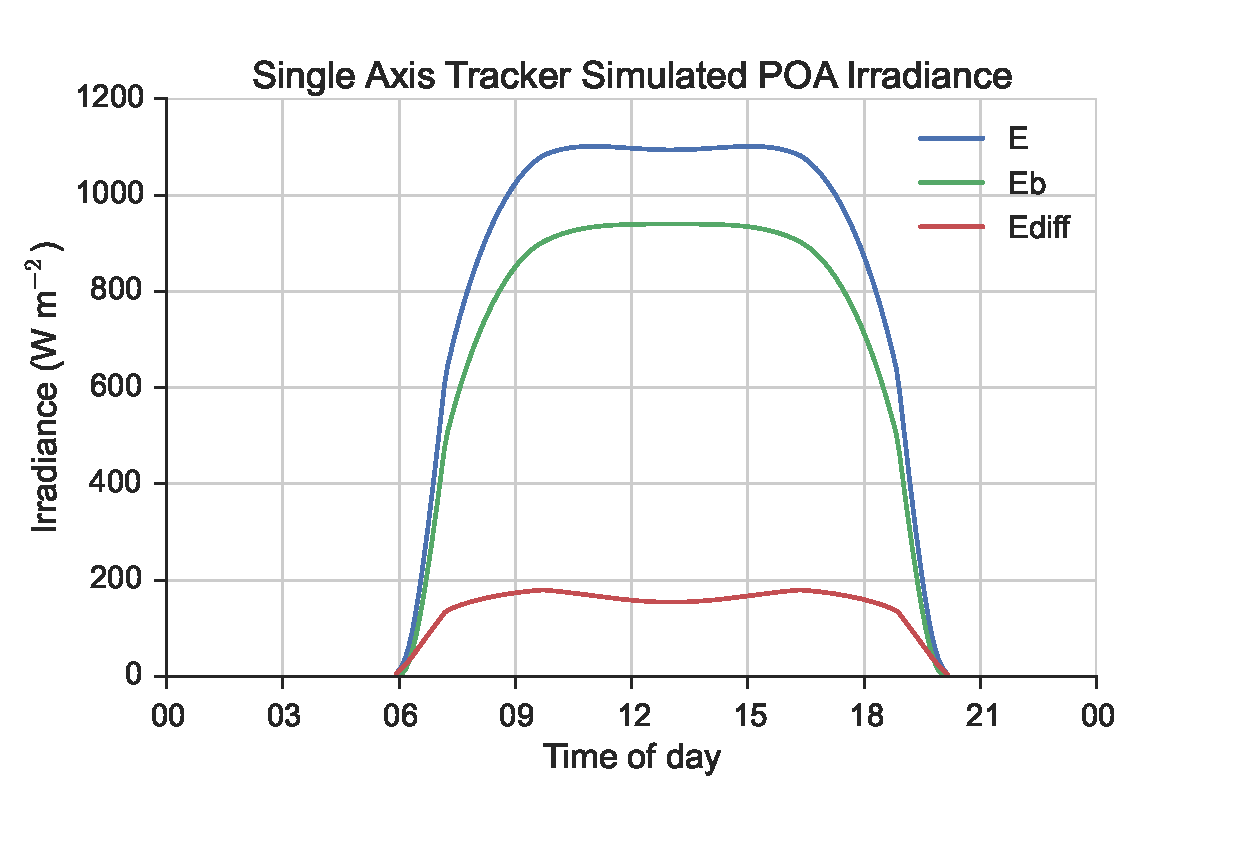
\includegraphics[width=9cm]{abq-tracker-irrad.eps}
\caption{\label{tracker}PVLIB-Python simulation of a single axis tracker, with backtracking, located near Albuquerque, NM, for June 1, 2015. The simulation outputs include (top) the angle of incidence (blue), panel surface azimuth (green), panel surface tilt (red), and angle of rotation about the tracking axis (purple) and (bottom) total plane of array irradiance (blue), beam component of plane of array irradiance (green), and diffuse plane of array irradiance (red). This example simulation used the Ineichen model to generate clear sky DNI, GHI, and DHI, the Hay-Davies model to generate the diffuse plane of array irradiance, and an isotropic ground diffuse model with an albedo of 0.25. This example may be compared to a similar simulation in the PVLIB-MATLAB documentation.}
\end{figure}

\begin{figure*}
\centering
\includegraphics[width=\textwidth]{fixed_sapm.eps}
\caption{\label{sapm}Simulation of a fixed-tilt PV system on April 1, 2015, in Tucson, AZ, using PVLIB-Python's implementation of the Sandia Array Performance Model. The top row of subfigures shows currents, voltages, and maximum power as a function of time of day, while the bottom row shows the same as a function of effective irradiance. PVLIB-Python was used to load the Sandia Module Database from NREL's website, calculate solar position, clear sky data, airmass, cell temperature, and module temperature, and finally run the Sandia Array Performance Model in 9 lines of code. Detailed simulation parameters may be found online \cite{pvlib-pvsc2015-github}.}
\end{figure*}

%\holmgren{if time/space permits, consider adding a table of modules and functions}

\subsubsection{Pythonic modification of design patterns}
Several design patterns existed in the Python package which were hold-overs from PVLIB-MATLAB. 
For example, PVLIB-MATLAB uses a struct to represent a location. 
Python does not have a C-like struct, but the initial PVLIB-Python attempted to keep the same pattern by creating a struct-like object.
By replacing the awkward Python version of a struct with a simple \texttt{pvlib.location.Location} class we obtained more readable and more functional code.
Objects of this \texttt{Location} class have added functionality such as more flexible constructors, better timezone handling, and nicer string representations.
Most importantly, the \texttt{Location} class can be extended by users for their own purposes.
For example, a user may define her own \texttt{SolarPlant} class that inherits from the \texttt{Location} class. 
\texttt{SolarPlant} objects could then interact with the rest of PVLIB in the same ways as \texttt{Location} objects, but also have additional user-defined attributes and functionality.
Additional changes include using making extensive use of \texttt{NaN} or \texttt{inf} values instead of setting values to 0, and applying PEP8 style and naming conventions \cite{pep8} to some of the code. 
Furthermore, most automatic input variable checking on design functions was removed as it is largely unnecessary in a Python environment and increased the complexity of the code. 

\subsubsection{Logging and debugging}
It is standard Python practice to use Python's built-in logging capabilities instead of print statements, so we replaced print statements with logging calls.
We are also now relying on built-in Python exceptions to alert the user to problems.
Using Python exceptions makes the PVLIB-Python library easier to integrate into a user's own programs.

\subsection{Accessibility for MATLAB users}
Rewriting the code to make it more pythonic leaves us with a significant problem: the package becomes less familiar to PVLIB-MATLAB users. 
We have attempted to lessen this problem in several ways.
First, we have provided extensive documentation, discussed more below, in the form of webpages and IPython notebooks that demonstrate where to find key functionality, how to tie together different components, and how to write good Python in the context of problems that PVLIB-MATLAB users are familiar with.
Second, wildcard import statements can be used to put the common PVLIB-MATLAB functions in the namespace of the Python script. 
For example, the TMY reading functions can be imported using \texttt{from pvlib.tmy import *}.
The PVLIB-Python GitHub community has discussed adding the ability to import all of the frequently used top-level functions using a command such as \texttt{from pvlib.api import *}.
Wildcard imports can sometimes lead to namespace problems and are often avoided in Python, but this functionality can provide PVLIB-MATLAB users with a more familiar interface while gradually becoming accustomed to Python design patterns.

\subsection{Testing and continuous integration}

Andrews et. al. described the need for both functional (does the code return a value or crash) and physical (does the code return the correct value) tests of the PVLIB code \cite{andrews}.
These tests are often called unit tests, in reference to the fact that there is ideally one test for each unit of code.
Here, a unit of code is typically a function, or a function called with a specific set of parameters.
PVLIB-Python now uses the \texttt{nose} package \cite{nosetests} to make writing tests faster and easier.
This package has been used to increase the testing coverage of the code to above 90\%.

Next, we adopted a continuous integration service, TravisCI, to automatically test the code every time that submits a pull request to merge their changes into another repository.
This helps to ensure that a contributor's changes to one part of the library does not inadvertently break another part of the library.
A comprehensive test suite coupled with continuous integration services also makes it relatively easy to test a library against many permutations of user environments.
As of June 1, 2015, we automatically test the PVLIB-Python package against Python versions 2.7 through 3.4, and pandas versions 0.13.1 through 0.16.1.

Writing new tests is a great way for new users to contribute to PVLIB-Python.
We particularly need physical tests, ideally benchmarked against other PV modeling programs.

\subsection{Installation}

Most popular Python packages use one of several tools to enable users to install the package into their Python environment.
Once installed, a Python package can be accessed regardless of the directory in which the user started the Python interpreter.
The original PVLIB-Python did not contain a usable installation script, which made using it and developing it more challenging.
We wrote a \texttt{setup.py} script to enable PVLIB-Python to be installed and to be developed more effectively.
We also added PVLIB-Python to the Python Package Index (PyPI), the most common resource for installing Python packages \cite{pvlib-pypi}.
PVLIB-Python can now be installed with a simple \texttt{pip install pvlib-python} command.
Future versions of PVLIB-Python will be installable using the \texttt{conda} package manager.


\subsection{Documentation}
Good documentation is essential to the success of any software.
We documented PVLIB-Python in two ways.
First, we created html and pdf documentation of the Python modules and functions.
Most of this documentation is an edited version of the PVLIB-MATLAB documentation.
We also documented the major differences between the Python and MATLAB projects.
PVLIB-Python uses the standard Python tools sphinx and numpydoc to build html and pdf documentation from function and module docstrings.
We use readthedocs.org to automatically build new versions of the documentation every time a change is made to the source code in the GitHub repository.
Figure \ref{rtd} shows a screenshot of the documentation homepage.
The second form of documentation is a collection of IPython notebooks.
IPython notebooks provide an informative combination of explanatory text and inline, executable code.
These notebooks can be viewed and downloaded at the GitHub project page or using the nbviewer.org tool. 
We strongly encourage the community to contribute to both forms of the PVLIB-Python documentation.
\begin{figure}
\includegraphics[width=9cm]{rtd.png}
\caption{\label{rtd}Screenshot of PVLIB-Python documentation homepage hosted at http://pvlib-python.readthedocs.org.}
\end{figure}


\section{Roadmap}

We propose one possible short-term roadmap for PVLIB-Python, and encourage the community suggest improvements.
We hope that PVLIB-Python administrative duties will rotate through the community on an annual to biannual basis.

\begin{enumerate}
\item Initial PVLIB-Python implementation released on GitHub under Sandia organization (completed in June, 2014) \cite{sandia-github}.
\item Establish a new GitHub organization, \texttt{pvlib}, to collaboratively administer the official PVLIB-Python project (completed February, 2015) \cite{pvlib-github}.
\item Put documentation on readthedocs.org \cite{pvlib-rtd} and use TravisCI (completed February, 2015).
\item First PVLIB-Python release on PyPI \cite{pvlib-pypi} (completed April, 2015).
\item Establish PVLIB-Python governance rules. Scientific Python packages, in particular IPython IPEP 29 \cite{ipython-gov}, may be a good resource.
\item Bring PVLIB-Python up to date with PVLIB-MATLAB 1.2.
\item Reach 100\% functional test coverage.
\item Release new version.
\item Develop and implement common physical tests for PVLIB-Python and PVLIB-MATLAB.
\item Encourage users to contribute new models, improve existing model implementations, testing, and documentation.
\item Release new version.
\item Rotate PVLIB-Python administrative duties.
\end{enumerate}


\section{Use cases}

We intend to establish a GitHub wiki to catalog PVLIB-Python use cases. Such a wiki may be modeled on the IPython project's \emph{A gallery of interesting IPython Notebooks} and \emph{Projects using IPython} \cite{ipythonwiki}. 


\section{Conclusion}
We described significant improvements to the PVLIB-Python package between the period June 2014 and May 2015 that make the library easier to use, easier to maintain, better tested, and better documented. 
Much more work remains, and we encourage readers to visit the GitHub project development website \cite{pvlib-github}.

% conference papers do not normally have an appendix

% use section* for acknowledgment
\section*{Acknowledgment}
The authors gratefully acknowledge Sandia National Laboratories for the initial development of PVLIB-MATLAB and PVLIB-Python and the ongoing contributions of many others to the project.
A list of PVLIB-Python contributors may be found on the GitHub repository \cite{pvlib-github} and in the online documentation \cite{pvlib-rtd}.
Sandia National Laboratories is a multi-program laboratory managed and operated by Sandia Corporation, a wholly owned subsidiary of Lockheed Martin Corporation, for the U.S. Department of Energy's National Nuclear Security Administration under contract DE-AC04-94AL85000.
WFH thanks the Department of Energy (DOE) Office of Energy Efficiency and Renewable Energy (EERE) Postdoctoral Research Award for support. 
ATL thanks the University of Arizona Renewable Energy Network for support.

% The following statement makes the two columns on the last page more
% or less of equal length.  Placement of this command is by trial and error.
\vfil\eject

% conference papers do not normally have an appendix


% use section* for acknowledgement



% trigger a \newpage just before the given reference
% number - used to balance the columns on the last page
% adjust value as needed - may need to be readjusted if
% the document is modified later
%\IEEEtriggeratref{8}
% The "triggered" command can be changed if desired:
%\IEEEtriggercmd{\enlargethispage{-5in}}

% references section

% can use a bibliography generated by BibTeX as a .bbl file
% BibTeX documentation can be easily obtained at:
% http://www.ctan.org/tex-archive/biblio/bibtex/contrib/doc/
% The IEEEtran BibTeX style support page is at:
% http://www.michaelshell.org/tex/ieeetran/bibtex/
\bibliographystyle{IEEEtran}
% argument is your BibTeX string definitions and bibliography database(s)
\bibliography{pvlib_pvsc_42}
%
% <OR> manually copy in the resultant .bbl file
% set second argument of \begin to the number of references
% (used to reserve space for the reference number labels box)
%\begin{thebibliography}{1}
%
%\bibitem{andrews}
%Robert W. Andrews, Joshua S. Stein, Clifford Hansen, and Daniel Riley, ``Introduction to the Open Source PV LIB for Python Photovoltaic System Modelling Package", \emph {in 40th IEEE Photovoltaic Specialist Conference}, 2014. 
%
%\bibitem{pvlibstein}
%J. S. Stein, ``The Photovoltaic Performance Modeling Collaborative (PVPMC)", \emph{Photovoltaic Specialists Conference}, 2012.

%\bibitem{acmpython}
%P. Guo, ``Python is Now the Most Popular Introductory Teaching Language at Top U.S. Universities", http://cacm.acm.org/blogs/blog-cacm/176450-python-is-now-the-most-popular-introductory-teaching-language-at-top-us-universities/fulltext Accessed January 22, 2015.

%\bibitem{pvlib-github}
%GitHub contributors, ``Sandia-Labs/PVLIB{\_}Python", https://github.com/Sandia-Labs/PVLIB{\_}Python Accessed January 22, 2015.

%\bibitem{uaren-pvlib}
%W. F. Holmgren, A. T. Lorenzo, and GitHub contributors, ``UARENForecasting/PVLIB{\_}Python", https://github.com/UARENForecasting/PVLIB{\_}Python Accessed January 22, 2015.
%
%\bibitem{zenofpython}
%T. Peters, ``PEP 20 -- The Zen of Python", https://www.python.org/dev/peps/pep-0020/ Accessed January 22, 2015.
%
%\bibitem{nosetests}
%nose contributors, https://nose.readthedocs.org/en/latest/ Accessed January 22, 2015.
%
%\bibitem{pythonic}
%M. Faassen, ``What is Pythonic?", http://blog.startifact.com/posts/older/what-is-pythonic.html Accessed January 22, 2015.
%
%\bibitem{pep8}
%G. van Rossum and N. Coghlan, ``PEP 8 -- Style Guide for Python Code", https://www.python.org/dev/peps/pep-0008/ Accessed January 22, 2015.
%
%\bibitem{ipython-gov}
%IPython IPEP 29 contributors, ``IPEP 29: Project Governance", https://github.com/ipython/ipython/wiki/IPEP-29\%3A-Project-Governance Accessed January 22, 2015.
%
%\bibitem{ipython-wiki}
%IPython wiki contributors, ``A gallery of interesting IPython Notebooks" and ``Projects using IPython", https://github.com/ipython/ipython/wiki/ Accessed January 22, 2015.

%\bibitem {Yamaguchi}
%M. Yamaguchi, A. Khan, S.J. Taylor, M. Imaizumi, T. Hisamatsu, and S. Matsuda, ``A detailed model to improve the radiation-resistance of Si space solar cells,\emph{Fundamentals of Solar Cells} vol. 46, pp. 2133-2138, 1999.
%
%\bibitem {Hovel}
%H. J. Hovel and J. M. Woodall, ``The effect of depletion region recombination currents on the efficiencies of Si and GaAs solar cells'', \emph {in 10th IEEE Photovoltaic Specialist Conference}, p. 25, 1973.
%
%\bibitem {Fahrenbruch}
%A. L. Fahrenbruch and R. H. Bube, \emph{Fundamentals of Solar Cells}, New York: Academic Press, 1983.

%\bibitem{IEEEhowto:kopka}
%H.~Kopka and P.~W. Daly, \emph{A Guide to \LaTeX}, 3rd~ed.\hskip 1em plus
%  0.5em minus 0.4em\relax Harlow, England: Addison-Wesley, 1999.

%\end{thebibliography}
%\smallskip
%Note: For the Summary paper submission only, references to the authors own work must be redacted to preserve the new double-blind reviewing requirements.





% that's all folks
\end{document}


